\section{Trình bày sơ đồ khối trong SFC}
Sơ đồ khối SFC  
\begin{figure}[H]
    \centering
    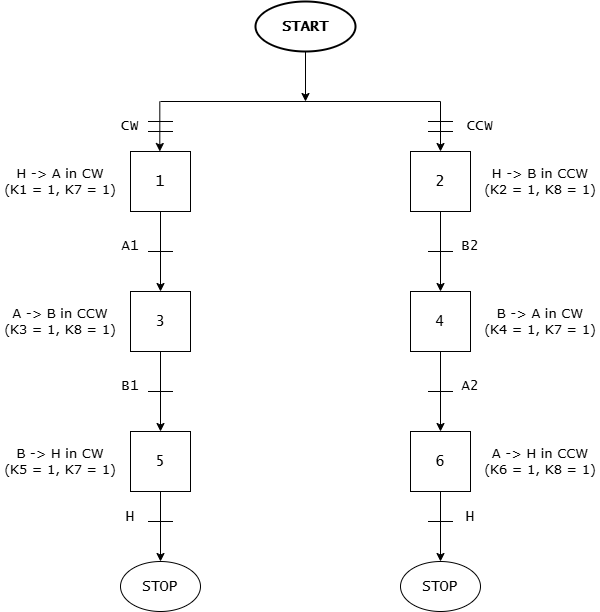
\includegraphics[width=0.9\textwidth]{pictures/SFC.png}
\end{figure}
Trong đó 2 nhánh lần lượt bắt đầu bằng CW, CCW thể hiện cho 2 nút bấm, 2 chế độ quay của bàn xoay.\\
Trong từng nhánh, các kí hiệu $Ki = 1 \,(i = 1, 2, \dots ,8)$ thể hiện trạng thái có điện của các cuộn dây $i$ tương ứng.
Trong đó $K7 = 1, \,K8 = 1$ lần lượt thể hiện cho chiều quay thuận và ngược chiều kim đồng hồ của động cơ.
\cleardoublepage